%&pdflatex
\documentclass{ecos}
\title{A new methodology to compute the Exergy Cost.\\ Part I: The Flow-Process Table}
\author{César Torres and Antonio Valero}
\address{CIRCE Institute. Universidad de Zaragoza, Spain\\
		 \mbox{email:ctorresc@unizar.es}}
\abstract{%
	The Exergy Cost theory was proposed in 1986 by Valero et al. in their “General theory of energy saving” (1986). This theory has been recognized as a powerful tool in the analysis of energy systems, and it has been applied to the assessment of alternatives for energy saving, local optimization, and thermoeconomic diagnosis.
	The paper introduces a new methodology, based on productive linear models, which provides new and more efficient algorithms to determine exergy costs and to analyze the cost formation process of products and wastes. This methodology consolidates the mathematical foundations of the Exergy Cost theory and enhances the computer implementation of the thermoeconomic  model.
	The keystone of this new approach is the Flow-Process table, which describes the  relationship “Processes uses flows to produce flows”, and characterizes the productive and dissipative structures of an energy system. 
}
\keywords{Exergy Cost Theory, Thermoeconomics, Productive models}
\subject{Paper for ECOS18 Conference}
\version{1.0}
\date{}

\begin{document}
\maketitle	
\section{Introduction}
According to the management theory, cost is defined as the amount of resources required to produce something or deliver a service. Energy cost accounting, in addition to a managerial technique for measure the consumption of energy resources, must provide a rational method for assessing the production costs and their impact on the environment.
There is a wide international consensus that exergy is the adequate thermodynamic property to use for cost assessment, at least for energy systems. Thermoeconomics combines economics and Second Law analysis applying the economic cost concept to exergy.

The problem of exergy costs allocation was formulated, in 1986 by Valero et al. \cite{Valero1986}, as follows: Given a system whose boundaries and level of aggregation that specifies the processes which constitute it have been defined. How to obtain the costs of all flows (energy carriers) that becomes interrelated in this structure?

Four conditions must be taken into consideration to solve this problem:
\begin{compactenum}[(i)]
	\item The defined boundaries are relatives to the system under study. Energy, raw materials, information, and labour resources used by the system must be specified.
	\item The level of aggregation provides a decomposition of the total irreversibility of the system among its processes or components. The level of aggregation chosen will affect the conclusions of the analysis. In fact, we do not have more information about the system than that defined by its aggregation level. The analyst should to disaggregate the system into processes and flows until the information could be used effectively. 
	\item The efficiency, as an indicator of process quality, must be used as physical criteria to allocate exergy costs. The exergy costs of the resources used by a process must be allocated to their products proportionally to its exergy content. 
	\item The system produces undesirable flows or wastes, and consumes external resources to produce and eliminate these wastes. The formation process of wastes must be analyzed, in order to determine the origin of waste flows and to make a correct cost allocation. 
\end{compactenum}

The Exergy Cost theory \cite{ECT93} (hereinafter ECT) provides rational and objective criteria to allocate cost based on the definition of efficiency of the processes which constitute the system. It has been recognized as a powerful tool in the analysis of energy systems, and it has been applied to the assessment of alternatives for energy saving, local optimization, and thermoeconomic diagnosis.

The algebraic method, provided by ECT, to calculate exergy costs has some drawbacks: From the mathematical viewpoint, the original ECT approach does not ensure the existence, uniqueness and positiveness of the solution. From software implementation viewpoint, the method has limitations and accuracy problems when deals with complex structures. Finally, the problem of waste cost allocation is not treated in a rigorous and general way.

The aim of this paper is to introduce a new methodology to compute exergy costs, which combines graph theory an linear models with the allocation rules of ECT. This methodology will provide a rigorous mathematical approach that gives solutions to the cost allocation problem formulated above.

From a theoretical viewpoint, an energy system is defined beforehand as a set of subsystems or thermodynamic processes linked to each other and to the environment by another set of mass, heat, and work flows, quantified by its exergies. In essence, it constitutes a flowsheet, as it is shown in \cref{fig1}. This example represents a gas turbine cycle (henceforth called TGAS) that uses natural gas (flow \#5) to produces 10 MW of electric power (flow \# 6) and evaporates 8 kg/s of water at 20 bar of pressure, partially recovering the residual heat of gases. The exergy flow \#8 is calculated as the difference between the exergy of the saturated steam and and the inlet water. Finally, the waste combustion gases are expelled through a stack (flow \#9). This flowsheet indicates also the system boundaries and the aggregation level. The exergy values of the plant flows are show in \cref{tab4}.  

\begin{figure}[h]
	\centering
	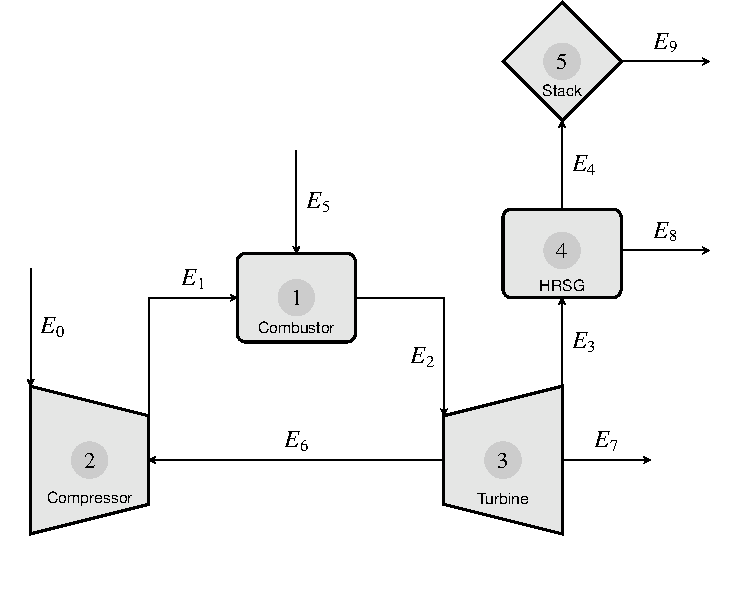
\includegraphics[width=0.65\linewidth]{tgas.pdf}
	\caption{Flowsheet of TGAS plant}
	\label{fig1}
\end{figure}

\section{The Productive Structure}
Industrial installations have a productive purpose. Their objective is to obtain one or several products by processing external resources. For each process of the system is necessary to identify the flow that constitute their product streams, and the flow  required to obtain them, called fuel streams \cite{Tsatsaronis1985,SPECO06}. Energy flows (e.g heat or work) appear at the process inlet as fuel streams, or at the process outlet as product streams. When working with mass streams, it is appropriate to operate with exergy differences associated with each energy transfer between inlet and outlet.

A fuel stream will consist of:
\begin{elist}
	\item One or several inflows that provide exergy to the process.
	\item Input and output flows belong to a mass flow stream that entering the process and leave it after transfer exergy to the process.
\end{elist}
A product stream will consist of:
\begin{elist}
	\item One or several outflows produced by the process.
	\item Output and input flows belong to a mass flow stream that entering the process and leave it after increasing it exergy.
\end{elist}

The exergetic efficiency of a process $u$ is defined as the ratio between the exergy obtained or product and the exergy supplied or fuel. It measures how reversible a process is. The inverse value is the exergy unit consumption, i.e, the amount of resources required per unit of product obtained:
\begin{equation}
k_u=\frac{F_u}{P_u} \ge 1
\end{equation}
where $F_u$ is the exergy provided by its fuel streams and $P_u$ is the exergy of its product streams. The second law states that the exergy of the fuels is bigger than the exergy of the products, and the difference is the irreversibility $I_u$ of the process.
\begin{equation}
\label{eq:fpi}
F_u - P_u = I_u \ge 0
\end{equation}

\begin{figure}[htpb]
	\begin{subfigure}{0.48\textwidth}
		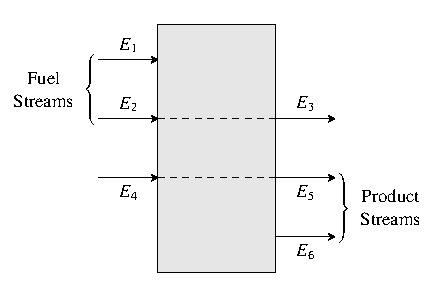
\includegraphics{ps1}
		\caption{Physical diagram} \label{fig2a}
	\end{subfigure} \hfill
	\begin{subfigure}{0.48\textwidth}
		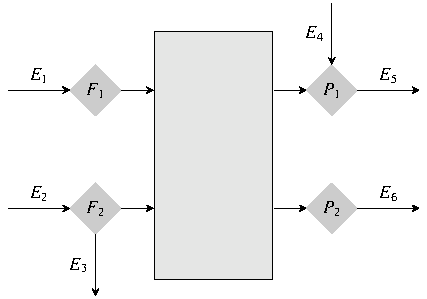
\includegraphics{ps2}
		\caption{Productive diagram} \label{fig2b}
	\end{subfigure}
	\caption{Physical and productive diagrams of a generic component}
	\label{fig2}
\end{figure}

Consider a generic component, as it is shown in \cref{fig2}, whose unit exergy consumption is defined as:
\begin{equation}
k=\frac{E_1 + (E_2 - E_3)}{E_6 + (E_5-E_4)}
\end{equation}
The objective of the process is to produce the flow $E_6$ and to increase the exergy of flow \#4 to $E_5$. For this purpose, two fuel streams are defined: the flow $E_1$ and the exergy transferred by the difference ${E_2-E_3}$. Flows 1, 2 and 3 are associated with the fuel streams meanwhile flows 4,5,6 to the product streams.

In the productive or logical diagram, the streams are represented by diamonds. They are not physical processes, but logical connectors between flows and processes, whose contains the information about the processes efficiency. \Cref{tab1} shows the definition of the fuel and product streams of each process in the case of TGAS plant. 

\begin{table}[H]
	\caption{Processes description and efficiency definition of TGAS plant}	
	\label{tab1}
	\begin{tabularx}{0.75\textwidth}{B{1.5cm}WZZ}
		\toprule
		Nr & Process & Fuel  & Product  \\ 
		\midrule
		1  & Combustor  & $E_5$     & $E_2-E_1$ \\ 
		2  & Compressor & $E_6$     & $E_1$     \\ 
		3  & Turbine    & $E_2-E_3$ & $E_6+E_7$ \\ 
		4  & HRSG       & $E_3-E_4$ & $E_8$     \\ 
		5  & Stack      & $E_4$     & $E_9$     \\ 
		\bottomrule 
	\end{tabularx} 
\end{table}

Let $\mathcal{V}=\left\{u_0,u_1,\ldots,u_n\right\}$ to be the set of the $n$ components or processes whose constitute the system, for a defined boundaries and level of aggregation. The component $u_0$ represents the environment. Let define $\mathcal{B}=\left\{b_1,\ldots,b_m\right\}$ as the set of the $m$ flows that interchange exergy between the processes.
Finally, let $\mathcal{L}=\{\ell_1,\ldots,\ell_{nr}\}$ to be the set of all the fuel and product streams of the system.

Each component of the system has several fuel and product streams, let  ${\mathcal{F}_u=\{f_1,\ldots,f_{l_u}\}}$ and ${\mathcal{P}_u=\{p_1,\ldots,p_{h_u}\}}$ to be the sets of fuel and product streams of the process $u$, where $l_u$ is the number of fuel streams, and $h_u$ the number of product streams of process $u$.
On the other hand, each stream $\ell \in \mathcal{L}$ could have several inputs and output flows. Let denote $\mathcal{E}_l$ and  $\mathcal{S}_l$ as the sets of input and output flows of the stream $\ell$.  A fuel stream must have at least one input flow, and a product stream must have at least one output flow. The environment has a product stream, whose output flows $\mathcal{S}_0$ are the external resources, and a fuel stream whose input flows are the system outputs $\mathcal{E}_0$.

\begin{figure}[htpb]
	\centering
	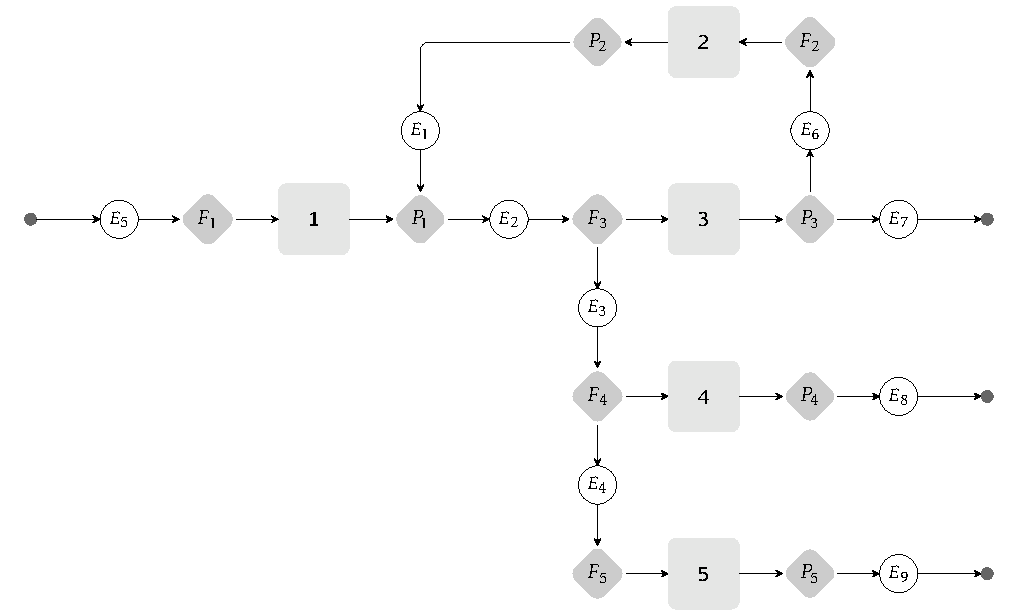
\includegraphics[width=0.98\linewidth]{tgasfp1}
	\caption{Productive structure graph of TGAS plant}
	\label{tgasfp}
\end{figure}

The productive structure could be represented as a directed graph, with three types of nodes: processes $(\mathcal{V})$, flows $(\mathcal{B})$ and streams $(\mathcal{L})$ , and four types of edges or relations: process-stream  $(\mathcal{F}_u)$, stream-process $(\mathcal{P}_u)$, flow-stream $(\mathcal{E}_l)$ and stream-flow $(\mathcal{S}_l)$. The productive structure graph for the TGAS plant is shown in \cref{tgasfp}, where processes are represented by squares and flows by circles.

Each stream $\ell \in \mathcal{L}$ has associated a measure corresponding to the exergy processed. Let denote $F_{u,l}$ as the exergy of the fuel stream $\ell$ of the process $u$, therefore
\begin{equation}
F_{u,l} = \sum_{i\in\mathcal{E}_l} E_i - \sum_{j\in\mathcal{S}_l} E_j \ge 0 \qquad \ell\in\mathcal{F}_u
\label{eq:fs}
\end{equation}
\label{eq2_3}
Similarly, in case of a product stream, let denote  $P_{u,l}$ as the exergy  product stream $\ell$ of the process $u$.
\begin{equation}
P_{u,l}=\sum_{j\in\mathcal{S}_l} E_i - \sum_{i\in\mathcal{E}_l} E_i \ge 0
\label{eq:ps}
\end{equation}
Finally, the fuel $F_u$ and product $P_u$ of each process $u$ is defined as the sum of their corresponding streams, and by \cref{eq:fpi}: $F_u \ge P_u$. 
\begin{equation}
F_u=\sum_{l\in\mathcal{F}_u} F_{u,l} > 0 \quad\text{and} \quad P_u=\sum_{l\in\mathcal{P}_u} P_{u,l} > 0
\end{equation}

\section{The Flow-Process Table}
The productive structure is based on the underlying idea that the processes of an energy system use flows to produce flows. The flow-process approach has two sides:

On the use side, the inflows of a fuel stream are used as resources of the process and additionally part of the exergy of the stream, not used by the process, becomes the output flows of the stream. Given a fuel stream $\ell$ of the process $u$, from \cref{eq:fs}, it leads:
\begin{equation}
\sum_{i\in\mathcal{E}_l} E_i = F_{u,l} + \sum_{j\in\mathcal{S}_l} E_j
\end{equation}
Let $\mathrm{FE}_{u,l}$ to be the input exergy of the stream $\ell$, then we define the input exergy ratio $x_i$ as:
\begin{equation}
x_i=\begin{cases}
\dfrac{E_i}{FE_{u,l}}& E_i>0 \quad \text{and} \quad i\in\mathcal{E}_l,\; \ell\in\mathcal{F}_u \\[1em]
\quad0&\text{otherwise}
\end{cases}
\end{equation}
therefore:
\begin{equation}
E_i = x_i \, F_{u,l} + x_i\sum_{j\in\mathcal{S}_l} E_j
\end{equation}
On the production side, the outflows of a stream come, part from the product of the process and optionally by flows that come from other processes, from \cref{eq:ps}, it leads:
\begin{equation}
\sum_{j\in\mathcal{S}_l} E_j = P_{u,l} + \sum_{i\in\mathcal{E}_l} E_i
\end{equation}
Let $\mathrm{PS}_{u,l}$ to be the output exergy of the stream and let $y_j$ to be the bifurcation ratio, defined as:
\begin{equation}
y_j=\begin{cases}
\dfrac{E_j}{PS_{u,l}}& E_j>0 \quad \text{and} \quad j\in\mathcal{S}_l,\; \ell\in\mathcal{P}_u \\[1em]
\quad0&\text{otherwise}
\end{cases}
\end{equation}
therefore:
\begin{equation}
E_j = y_j \, P_{u,l} + y_j\sum_{i\in\mathcal{E}_l} E_i
\end{equation}
These relationships can be written in matrix form as follows:

Let  $\mbt{F}$ to be a  $m \times n$ matrix, whose elements, $f_{iu}=x_i\,F_{u,l},\, i\in\mathcal{E}_l, \, \ell\in\mathcal{F}_u$, represent the exergy  of the input flow $i$ used as fuel of process $u$.

Similarly, let $\mbt{P}$ to be a $n \times m$ matrix , whose elements, $p_{uj}=y_j\,P_{u,l},\, j\in\mathcal{S}_l, \, \ell\in\mathcal{P}_u$, represent the exergy value of the output flow $j$ used as product of process $u$.
 
Finally, let $\mbt{V}$ to be a $m \times m$, whose elements $v_{ij}$ represent the exergy of the input flow $i\in\mathcal{E}_u$ becomes the output flow $j\in\mathcal{S}_u$. These elements are defined only if the stream has both input and outputs flows.
\begin{equation}
v_{i,j}=\begin{cases}
\;x_i\,E_j & i\in\mathcal{E}_l,\, j\in\mathcal{S}_l,\, \ell\in\mathcal{F}_u\\[1em]
\;y_j\,E_i & i\in\mathcal{E}_l,\, j\in\mathcal{S}_l,\, \ell\in\mathcal{P}_u\\
\end{cases}
\end{equation}
The vector $\bm{\nu}_0 (1 \times m)$ contains the exergy values of the external resources, and the vector $\bm{\omega}_0 (m \times 1)$ contains the exergy values of the system outputs:
\begin{equation}
\nu_{0,i}=\begin{cases}
\;E_i & i\in\mathcal{S}_0 \\
\;0   & \text{otherwise}
\end{cases}
\qquad\qquad
\omega_{0,i}=\begin{cases}
\;E_i & i\in\mathcal{E}_0 \\
\;0   & \text{otherwise}
\end{cases}
\end{equation}
This information can be summarized by the flow-process table, see \cref{fig4}, which describes the relationship \emph{process uses flows to produce flows}.
\begin{figure}[H]
	\renewcommand{\arraystretch}{1.2}
	\begin{subtable}{0.40\textwidth}
		\begin{tabular}{c|c|B{1.4cm}|B{1.4cm}|c|}
			\multicolumn{1}{c}{}& \multicolumn{1}{c}{} & \multicolumn{2}{c}{\small outputs}& \multicolumn{1}{c}{} \\
			\cline{2-5}
			& & $\bm{0}$ & $\bm{\nu}_0$ & $F_T$ \\     
			\cline{2-5}
			\parbox[t]{3mm}{\multirow{6}{*}{\rotatebox[origin=c]{90}{\small inputs}}}
			& & & & \\
			& $\bm{0}$ & $\bm{0}$ & [\vm{P}] & \vm{P} \\ 
			& & & & \\
			\cline{2-5}
			& & & & \\
			& $\bm{\omega}_0$ & [\vm{F}] & [\vm{V}] & \vm{E} \\ 
			& & & & \\
			\cline{2-5}
			& $P_T$ &\vm{F} &\vm{E} & \\
			\cline{2-5}
		\end{tabular}
		\caption{Flow-Process Table} \label{tab2a}
	\end{subtable} \hfill
	\begin{subtable}{0.40\textwidth}
		\begin{tabular}{c|c|B{1.4cm}|B{1.4cm}|c|}
			\multicolumn{1}{c}{}& \multicolumn{1}{c}{} & \multicolumn{2}{c}{\small outputs}& \multicolumn{1}{c}{} \\
			\cline{2-5}
			& & $\bm{0}$ & $\bm{0}$ & $\bm{0}$ \\     
			\cline{2-5}
			\parbox[t]{3mm}{\multirow{6}{*}{\rotatebox[origin=c]{90}{\small inputs}}}
			& & & & \\
			& $\bm{0}$ & $\bm{0}$ & $\bm{0}$ & $\bm{0}$ \\ 
			& & & & \\
			\cline{2-5}
			& & & & \\
			& $\bm{0}$ & [\vm{R}] & $\bm{0}$ &  $\bm{\omega}_r$  \\ 
			& & & & \\
			\cline{2-5}
			& $\bm{0}$ &\vm{R} & $\bm{0}$ & \\
			\cline{2-5}
		\end{tabular}
		\caption{Waste-Process Table} \label{tab2b}
	\end{subtable}
	\caption{Flows-Processes and Waste-Process Tables}
	\label{fig4}	
\end{figure}
Let \vm{F} and \vm{P} to be $n\times1$ vectors, whose elements are the fuel and product of the processes, and \vm{E} a $m\times1$ vector, whose elements are the exergy of the flows. We will denote by $\tvm{u}_n\equiv(1,\ldots,1)$ the unitary row vector of dimension $n$.
The submatrices of the flow-process table verify the following properties:
\begin{align}
\vm{F}&=\tvm{u}_m\,[\vm{F}] \\
\vm{P}&=[\vm{P}]\,\vm{u}_m \\
\vm{E}&=\bm{\omega}_0 + [\vm{F}]\,\vm{u}_n + [\vm{V}]\,\vm{u}_m = \tm\bm{\nu}_0 + \tm[\vm{P}]\,\vm{u}_n + \tm[\vm{V}]\,\vm{u}_m
\end{align}
The rows of \cref{tab2a} reflect the use inputs of flows in processes, meanwhile the columns the output flows produced by process. In \cref{tab3} it is shown the flow-process table corresponding to the TGAS plant. Observe that the lower-left part of the table $\mbt{F}$ contains the fuel definition of the processes, and the upper-right part $\mbt{P}$ contains the product definition. The lower-right part $\mbt{V}$ is used to close the input-output flows balance.

\begin{table}[H]
	\centering
	\caption{Flow-Process table of TGAS plant}
	\resizebox{\textwidth}{!}{%
		\begin{tabular}{|c|c|UUVVU|UVUUUUUUU|}
			\hline
			& $F_0$    & $F_1$    & $F_2$    & $F_3$    & $F_4$    & $F_5$    & $E_1$    & $E_2$    & $E_3$    & $E_4$    & $E_5$    & $E_6$    & $E_7$    & $E_8$    & $E_9$ \\
			\hline
			$P_0$   & 0     & 0     & 0     & 0     & 0     & 0     & 0     & 0     & 0     & 0     & $E_5$   & 0     & 0     & 0     & 0 \\
			\hline
			$P_1$   & 0     & 0     & 0     & 0     & 0     & 0     & 0     & $E_2-E_1$ & 0     & 0     & 0     & 0     & 0     & 0     & 0 \\
			$P_2$   & 0     & 0     & 0     & 0     & 0     & 0     & $E_1$   & 0     & 0     & 0     & 0     & 0     & 0     & 0     & 0 \\
			$P_3$   & 0     & 0     & 0     & 0     & 0     & 0     & 0     & 0     & 0     & 0     & 0     & $E_6$   & $E_7$   & 0     & 0 \\
			$P_4$   & 0     & 0     & 0     & 0     & 0     & 0     & 0     & 0     & 0     & 0     & 0     & 0     & 0     & $E_8$   & 0 \\
			$P_5$   & 0     & 0     & 0     & 0     & 0     & 0     & 0     & 0     & 0     & 0     & 0     & 0     & 0     & 0     & $E_9$ \\
			\hline
			$E_1$   & 0     & 0     & 0     & 0     & 0     & 0     & 0     & $E_1$   & 0     & 0     & 0     & 0     & 0     & 0     & 0 \\
			$E_2$   & 0     & 0     & 0     & $E_2-E_3$ & 0     & 0     & 0     & 0     & $E_3$   & 0     & 0     & 0     & 0     & 0     & 0 \\
			$E_3$   & 0     & 0     & 0     & 0     & $E_3-E_4$ & 0     & 0     & 0     & 0     & $E_4$   & 0     & 0     & 0     & 0     & 0 \\
			$E_4$   & 0     & 0     & 0     & 0     & 0     & $E_4$   & 0     & 0     & 0     & 0     & 0     & 0     & 0     & 0     & 0 \\
			$E_5$   & 0     & $E_5$   & 0     & 0     & 0     & 0     & 0     & 0     & 0     & 0     & 0     & 0     & 0     & 0     & 0 \\
			$E_6$   & 0     & 0     & $E_6$   & 0     & 0     & 0     & 0     & 0     & 0     & 0     & 0     & 0     & 0     & 0     & 0 \\
			$E_7$   & $E_7$   & 0     & 0     & 0     & 0     & 0     & 0     & 0     & 0     & 0     & 0     & 0     & 0     & 0     & 0 \\
			$E_8$   & $E_8$  & 0     & 0     & 0     & 0     & 0     & 0     & 0     & 0     & 0     & 0     & 0     & 0     & 0     & 0 \\
			$E_9$   & $E_9$  & 0     & 0     & 0     & 0     & 0     & 0     & 0     & 0     & 0     & 0     & 0     & 0     & 0     & 0 \\			
			\hline
		\end{tabular}
	}%
	\label{tab3}%
\end{table}%

\subsection{Waste Flows and Dissipative Processes}
In any energy system, along with final products \cite{Agudelo12}, does appear flows were not pretended to obtain, which are called \emph{wastes} or residues.  These flows are mostly caused by technological limitations imposed by the equipment and processes of the plant.
Waste flows still have exergy cannot be recovered by the system. We have spent resources to produce and to dispose of them. If the wastes are formed in the same process they output, they could be considered as exergy losses and add to the process irreversibility, but usually, they output in different processes they are formed. For instance, the combustion gases output the stack are produced in the combustion chamber.

For a proper allocation, we must follow their formation process and assess the cost of their formation and disposal to the processes in which they are produced. In parallel to the cost formation process of the products, there is a cost formation process of wastes.

Let denote $\mathcal{R}$ as the subset of output system flows $\mathcal{E}_0$ whose are wastes of the system. Therefore, the system outputs could be split into two parts, $\bm{\omega}_0=\bm{\omega}_s+\bm{\omega}_r$.
Let $\bm{\omega}_r$ be a  $m \times 1$ vector which contains the exergy of the waste flows and $\bm{\omega}_s$ a $m \times 1$ vector which contains the exergy of the final products:
\begin{equation}
\omega_{r,i}=\begin{cases}
\;E_i&i\in \mathcal{E}_0\cup\mathcal{R} \\
\;0 & \text{otherwise}
\end{cases}
\qquad \qquad
\omega_{s,i}=\begin{cases}
	\;E_i&i\in \mathcal{E}_0\cup\bar{\mathcal{R}} \\
	\;0 & \text{otherwise}
\end{cases}
\end{equation}

Let \mbt{R} to be a $n \times n$ matrix, called \emph{waste-process table}, whose elements $r_{iu}$ represent the exergy of waste flow $i\in\mathcal{R}$ generated by the process u.
This matrix verify the following properties:
\begin{align}
\bm{\omega}_r &=[\vm{R}]\,\vm{u}_n \\
\vm{R} &=\tm\mbt{R}\,\vm{u}_m
\end{align}
where $\vm{R}$ is a $1\times n$ vector whose elements contain the exergy of the wastes generates by each process. The waste-process table, see \cref{fig2b}, describes the cost formation process of waste and it is integrated as an additional layer of the productive structure.

In the case of TGAS, there is only a waste flow: $E_9$. Its exergy has two components: thermal, because the  temperature of the gases is higher than the environment temperature, and chemical because the composition of gases is different than the reference environment. Moreover, the combustion gases contains harmful substances that must be removed, and for this purpose, additional exergy resources must be required. The origin of the thermal and chemical exergy of gases is caused in the combustion process, therefore the cost of these wastes must be charge to the combustor. Then, matrix $\mbt{R}$ has only one entry $r_{9,1}=E_9$.

There are not unique criteria to determine the values of the \mbt{R} table. In general, a deep thermodynamic analysis of the plant processes is required to identify where the wastes are formed. Several works \cite{Frangopoulos87,Gonzalez03,Mendes17} analyse the waste flow cost allocation problem from different viewpoints.

\section{The Fuel-Product Rules of Cost Allocation}
Given an energy system whose productive structure has been specified, the exergy cost of a flow of that system as the amount exergy required to produce this flow.

Let denote $E_i^*$ the exergy cost of the system flow $i$, and $k_i^*$ the corresponding unit exergy cost. The exergy cost of a stream $\ell$ is defined as:
\begin{align}
F_{u,\ell}^{*}&=\sum_{i\in\mathcal{E}_l}{E_i^*}-\sum_{j\in\mathcal{S}_l}{E_j^*} \qquad \ell\in\mathcal{F}_u \\
P_{u,\ell}^{*}&=\sum_{j\in\mathcal{S}_l}{E_j^*}-\sum_{j\in\mathcal{E}_l}{E_i^*} \qquad \ell\in\mathcal{P}_u
\end{align}
and the exergy cost of fuel and product of a generic process $u$, is defined as the sum of the fuel or product streams of the process:
\begin{equation}
F_{u}^{*}=\sum_{l\in\mathcal{F}_u}{F_{u,\ell}^{*}} \qquad \qquad
P_{u}^{*}=\sum_{l\in\mathcal{P}_u}{P_{u,\ell}^{*}}
\end{equation}
The exergy cost of a flow cannot be measured as a physical magnitude of a flow stream as temperature or pressure; it depends on the system structure. The cost value of an individual flow in a given structure is senseless, but a set of interrelated costs values, which must be determined simultaneously, does. To find out their values, a set of propositions was proposed by the exergy cost theory \cite{Valero1986}:

\paragraph{FP1 Rule:} The exergy cost is relative to the system boundaries. In the absence of external assessment, the exergy costs of the flows entering the system equal their exergy. 
\begin{equation}
\label{eq:fprule1}
E_i^* = E_{i} \quad i\in\mathcal{S}_0 \tag{FP1}
\end{equation}
This indicates that, for the given boundaries of the system, the entering flows have no irreversibility. For this reason, selecting an appropriate limit of the system is fundamental for the analysis.
\paragraph{FP2 Rule:} The exergy cost is a conservative property. All the cost associated to a process, both resources $F_u^*$, and wastes $R_u^*$ must be assessed to the production costs.
\begin{equation}
\label{eq:fprule2}
P_{u}^{*}=F_{u}^{*}+R_{u}^{*} \quad u\in\mathcal{V} \tag{FP2}
\end{equation}
\paragraph{FP3 Rule:} The cost of the process irreversibility must be allocated to their products and distributed proportionally to their exergies.
\begin{elist}
	\item All the product streams of a process have the same unit exergy cost:
	\begin{equation}
	\label{eq:fprule3p}
	\frac{{P_u^*}}{P_u}=\frac{P_{u,l}^{*}}{P_{u,l}} \quad \ell\in\mathcal{P}_u \tag{{FP3P}}
	\end{equation}
	\item All the outputs of a product stream have the same unit exergy cost:
	\begin{equation}
	\label{eq:fprule3ps}
	k_j^*=\sum_{h\in\mathcal{S}_l}{y_h k_h^*} \quad j\in\mathcal{S}_l, \; \ell\in\mathcal{P}_u \tag{FP3PS}
	\end{equation}
	\item All the outputs of a fuel stream have the same unit cost equal to the average unit cost of the input flows of the stream:
	\begin{equation}
	\label{eq:fprule3f}
	k_j^* = \sum_{h\in\mathcal{E}_l}{x_h k_h^*} = \frac{F_{u,l}^*}{F_{u,l}} \quad j\in\mathcal{S}_l, \; \ell\in\mathcal{F}_u \tag{FP3F}
	\end{equation}
\end{elist}
These allocating criteria are based, exclusively, on the productive structure definition of the system. 
\paragraph{FP4 Rule:} The costs of waste flows must be allocated to the processes that have generated them.
\begin{equation}
\label{eq:fprule4}
R_u^*=\sum_{i\in\mathcal{R}}{k_i^* \, r_{iu}} \quad u\in\mathcal{V}_P \tag{FP4}
\end{equation}

The Fuel-Product rules of the Exergy Cost theory provide a set of rational rules based on thermodynamic criteria and the productive purpose. In the next section, we will prove that the Fuel-Product rules are necessary and sufficient conditions to unequivocally determine the exergy cost of all flows of a defined energy system.

\section{The Exergy Cost Equations}
Let $\vm{F}^*$ and $\vm{P}^*$ to be $n\times1$ vectors, whose elements are the exergy cost of fuel and product of the processes, and $\vm{E}^*$ a $m\times1$ vector, whose elements are the exergy cost of the flows.
The Fuel-Product rules could be expressed in terms of the elements of the flow-process table, by means of the following equations:
\begin{align}
\vm{E}^{*}&=\bm{\nu}_0+\tm\mbt{V}\,\vm{k}^{*}+\tm\mbt{P}\,\vm{c}_P \label{eq:ecta}\\
\vm{P}^{*}&= \tm\mbt{F}\,\vm{k}^{*}+ \tm\mbt{R}\,\vm{k}^{*} \label{eq:ectb}
\end{align}
To prove \cref{eq:ecta}, we need to verify that for all output flows:
\begin{equation}
\label{eq:ectsca}
E_{j}^{*}=\nu_{0j}+\sum_{u=1}^{n}{k_{P,u}^{*}\,p_{kj}+\sum_{i=1}^{m}{k_{i}}^{*}\,v_{ij}} \quad j\in\mathcal{B}
\end{equation}
\begin{enumerate}[i)]
	\item if $j\in\mathcal{S}_0$, by \ref{eq:fprule1} rule: $E_j^*=E_j$
	\item if $j\in\mathcal{S}_l$ and $\ell\in\mathcal{F}_u$, \cref{eq:ectsca} becomes:
	\[
	E_j^*=\sum_{i\in\mathcal{E}_l}{k_i^*\,x_i\,E_j}
	\]
	by \ref{eq:fprule3f} rule, it leads:
	\[
	k_j^*=\sum_{i\in\mathcal{E}_l}{k_i^*\,x_i}
	\]
	therefore, $k_j^*\,E_j=E_j^*$ and verify \cref{eq:ectsca}.
	\item if $j\in\mathcal{S}_l$ and $\ell\in\mathcal{P}_u$, \cref{eq:ectsca} becomes:
	\[
	E_j^*=k_{P,u}^*\,P_{u,l}\,y_j+\sum_{i\in\mathcal{E}_l}{k_i^*\,E_i\,y_j} 
	\]
	then, by rule \ref{eq:fprule3p}, it leads:
	\[
	k_{P,u}^*\,P_{u,l}\,y_j+\sum_{i\in\mathcal{E}_l}{k_i^*\,E_i\,y_j}=
	y_j\left(P_{u,l}^{*}+\sum_{i\in\mathcal{E}_l}{E_i^*}\right)=y_j\,\sum_{h\in\mathcal{S}_l}{E_h^*}
	\]
	and applying \ref{eq:fprule3ps} rule \cref{eq:ecta} is proved:
	\[
	y_j\,\sum_{h\in\mathcal{S}_l}{E_h^*}=E_j^*
	\]
\end{enumerate}
To demonstrate \cref{eq:ectb}, first, we prove that $\vm{F}=\vm{k}^*[\vm{F}]$, or equivalently:
\begin{equation}
F_u^*=\sum_{i=1}^{m}{k_i^* f_{iu}}=\sum_{l\in\mathcal{F}_u}{\sum_{i\in\mathcal{E}_l}{k_i^* x_i F_{u,l}}}
\end{equation}
then, by rule \ref{eq:fprule3f}:
\[
\frac{F_{u,l}^*}{F_{u,l}}=\sum_{i\in\mathcal{E}_l}{k_i^*x_i}
\]
and therefore:
\[
\sum_{l\in\mathcal{F}_u}{\sum_{i\in\mathcal{E}_l}{k_i^* x_i F_{u,l}}=\sum_{l\in\mathcal{F}_u}{F_{u,l}^*}}=F_u^*
\]
Finally, applying rules \ref{eq:fprule2} and \ref{eq:fprule4}, the equation \eqref{eq:ectb} is satisfied.
Note than the four FP rules are required to build equations \cref{eq:ecta,eq:ectb}. They provide a set of $m+n$ equations with $m+n$ unknowns, which determines the exergy costs of flows and products: $\vm{E}^*$ and $\vm{P}^*$.

\subsection{Exergy Costs Calculation}
\Cref{eq:ecta,eq:ectb} obtained above, let to determine the exergy costs for a given system state.

Let $\bm{\alpha}_F$ be a $m\times n$~matrix  so that: ${[\vm{F}]=\hat{\vm{E}}\,\bm{\alpha}_F}$, which verifies
\footnote{We denote by $\hat{\vm{x}}\equiv\text{diag}\{x_1,\ldots,x_n\}$, the diagonal matrix built  by a vector $\vm{x}$.}:
\begin{equation}
\vm{F}=\tm\bm{\alpha}_F\,\vm{E}
\end{equation}
Similarly, let $\bm{\alpha}_R$ to be a  $m\times n$~ matrix, so that: ${\mbt{R}}=\hat{\vm{E}}\,\bm{\alpha}_R$, which verifies: 
\begin{equation}
\vm{R} = \tm\bm{\alpha}_R \, \vm{E}
\end{equation}
Let  ${\bm{\beta}_P}$ to be a $ n \times m$~matrix , so that: ${\mbt{P}=\hat{\vm{P}}\,\bm{\beta}_P}$.
Finally, let \vm{B} to be a  $m \times m$ matrix so that: ${\mbt{V}=\hat{\vm{E}}\,\vm{B}}$.

These matrices are obtained by scaling the rows of the flow-process table by the corresponding exergy flows, and contains exergy distribution ratios. They verify:
\begin{align}
&\bm{\beta}_P\,\vm{u}_m = \vm{u}_n \label{eq:ectar}\\ 
&\bm{\alpha}\, \vm{u}_n + \vm{B}\,\vm{u}_m + \vm{a}_P= \vm{u}_m \label{eq:ectbr}
\end{align}
where $\bm{\alpha}=\bm{\alpha}_F+\bm{\alpha}_R$, and $\vm{a}_P$ is a $m \times 1$ vector, whose elements indicate if a flow is a final product:
\begin{equation}
a_{P,i}=\begin{cases}
\;1 & \text{if}\quad i\in\mathcal{E}_0 \cap \bar{\mathcal{R}} \\
\;0 & \text{otherwise}
\end{cases}
\end{equation}
Putting these matrices into \cref{eq:ecta,eq:ectb}, it leads the following relations:
\begin{align}
\vm{E}^{*}&=\bm{\nu}_0+\tvm{B}\,\vm{E}^{*}+\tm\bm{\beta}_{P}\,\vm{P}^{*} \label{eq:rda}\\
\vm{P}^{*}&=\tm\bm{\alpha}\vm{E}^{*} \label{eq:rdb}
\end{align}
and substituting \cref{eq:rdb} into \cref{eq:rda}, the following system of $m$ equations with $m$ unknowns is obtained, to determine the exergy cost of flows $\vm{E}^*$:
\begin{equation}
\label{eq:ectsol}
\tm\left(\vm{U}_m-\vm{B}-\bm{\alpha}\bm{\beta}_P\right)\vm{E}^*=\bm{\nu}_0
\end{equation}
To demonstrate that \eqref{eq:ectsol} has a unique solution, we will prove that $\vm{B}+\bm{\alpha}\bm{\beta}_P$ is a productive matrix (see Appendix part II), or equivalently that:
\[
\left(\vm{B}+\bm{\alpha}\bm{\beta}_P\right)\vm{u}_m \le \vm{u}_m
\]
From \cref{eq:ectar,eq:ectbr}, we get: $\left(\vm{B}+\bm{\alpha}\bm{\beta}_P\right)\vm{u}_m = \vm{u}_m - \vm{a}_P \le \vm{u}_m$. Therefore, if a energy system has final products, the exergy costs of the flows can be unequivocally determined by:
\begin{equation}
\vm{E}^*=\tm\mopsc{E}\bm{\nu}_0\,\qquad\text{where}\quad\mopsc{E}\equiv\left(\vm{U}_m-\vm{B}-\bm{\alpha}\bm{\beta}_P\right)^{-1}
\end{equation}
Moreover, matrix $\mopsc{E}$ is definite positive, i.e, all its elements are non-negative. Therefore, the exergy costs are always non-negatives because exergy is a non-negative magnitude.

\subsection{The Irreversibility-Cost Formula}
The equations of the flow-process model, could be written in terms of the matrices defined above:
\begin{align}
&\vm{E}=\bm{\nu}_0+\tm\bm{\beta}_P\vm{P}+\tvm{B}\,\vm{E} \label{eq:erda}\\
&\vm{F}+\vm{R}=\tm\bm{\alpha}\vm{E} \label{eq:erdb}
\end{align}
Applying the exergy balance equation \cref{eq:fpi} in vectorial form to \cref{eq:erdb}, it leads: ${\vm{P}=\tm\bm{\alpha}\vm{E}-\vm{I}-\vm{R}}$. Substituting into \cref{eq:erda}:
\begin{equation}
\bm{\nu}_0=\tm\left(\vm{U}_m-\vm{B}-\bm{\alpha}\bm{\beta}_P\right)\vm{E}+\tm\bm{\beta}_P\left(\vm{I}+\vm{R}\right)
\end{equation}
and right multiplying both sides by $\tm\mopsc{E}$:
\begin{equation}
\label{eq:icff}
\vm{E}^*=\vm{E}+\tm\mopsc{E}\,\tm\bm{\beta}_P\left(\vm{I}+\vm{R}\right)
\end{equation}
\Cref{eq:icff}, called \emph{irreversibility cost formula}, is essential to understand the process of cost formation. It shows the exergy cost of a flow equals its exergy plus the sum of all exergy destroyed (irreversibility, losses and wastes) during the production process of that flow. In the above equation $\bm{\beta}_P\,\left(\vm{I}+\vm{R}\right)$ represents the local exergy losses assesses to each output flow, and then the cost operator $\mopsc{E}$  distribute this irreversibility cost to the rest of processes of the system.

Because the last term in \cref{eq:icff} is  positive, then the exergy cost of a flow is always greatest or equal to its exergy: $E_i^* \ge E_i$ for each $i$. The equality is satisfied only if there is no irreversibility in the production of such flow. It is the case of the external resources, whose cost is equal to its exergy. 

This property is also extended to the fuel and product streams. Multiplying both sides of \cref{eq:icff} by $\tm\bm{\alpha}_F$, it leads: $\vm{F}^*\ge\vm{F}$, therefore, {$k_{F,u}^{*}\ge 1$} and {$k_{P,u}^{*}\ge k_u$} for each processs $u$.

\Cref{tab4} shows the exergy cost of flows for the TGAS plant.
The first row contains the exergy values of flows, the next five rows the contribution of the irreversibility of each process to the exergy cost, and the sixth row the contribution of the wastes. In this case, the exergy costs of the gases dissipated in the stack represent 5.93\% of the cost of the flows.

\begin{table}[H]
	\small
	\caption{Direct exergy cost of flows for TGAS plant, using irreversibility cost formula}
	\begin{tabular}{crrrrrrrrr}
		\toprule
		Flow & 1 & 2 & 3 & 4 & 5 & 6 & 7 & 8 & 9 \\
		\midrule
		$E$     & 9512.0 & 32990.0 & 11707.0 & 2173.0 & 36620.0 & 10225.0 & 10000.0 & 6666.0 & 2173.0 \\
		\midrule
		$I_1$    & 7050.2 & 21616.0 & 7670.8 & 1423.8 & 0.0   & 7050.2 & 6895.0 & 6247.0 & 1423.8 \\
		$I_2$    & 1095.5 & 1172.7 & 416.2 & 77.2  & 0.0   & 382.5 & 374.1 & 338.9 & 77.2 \\
		$I_3$    & 821.8 & 879.8 & 312.2 & 57.9  & 0.0   & 821.8 & 803.7 & 254.3 & 57.9 \\
		$I_4$    & 0.0   & 0.0   & 0.0   & 0.0   & 0.0   & 0.0   & 0.0   & 2868.0 & 0.0 \\
		$I_5$    & 0.0   & 0.0   & 0.0   & 0.0   & 0.0   & 0.0   & 0.0   & 0.0   & 0.0 \\
		$R$     & 1165.7 & 3574.2 & 1268.3 & 235.4 & 0.0   & 1165.7 & 1140.1 & 1032.9 & 235.4 \\
		\midrule
		$E^*$ & 19645.2 & 60232.7 & 21374.5 & 3967.4 & 36620.0 & 19645.2 & 19213.0 & 17407.0 & 3967.4 \\
		\midrule
		$k^*$ & 2.0653  & 1.8258	& 1.8258  &	1.8258 & 1.0000	& 1.9213 & 1.9213 & 2.6113 & 1.8258 \\
		\bottomrule
	\end{tabular}%
	\label{tab4}%
\end{table}%

\subsection{The Generalized Exergy Cost}
As we are mentioned above, the exergy cost is relative to  to the system boundaries.
Therefore, we will distinguish between the thermodynamic system that constitutes the installation and its environment. Exergy cost, also called \emph{direct exergy cost} only takes the irreversibility of the processes inside the boundaries of the system into account. 

From the point of view of natural resources management, the boundary should reach the level of extraction of non-renewable resources from nature. The exergy cost of natural gas processed in a gas turbine will be higher than its exergy due to the different processes: extraction, storage and transportation that have been required for it to be used.  Moreover, direct exergy cost has not considered the fact that the units that form an installation are functional products, and they have their own exergy cost $Z$, because to keep them in operation, additional exergy will be required.   
This kind of analysis is possible, for example, with the application of the thermoecological cost (TEC). According to J. Szargut \cite{Szargut2005}, the TEC is defined as the cumulative consumption of non-renewable exergy connected with the fabrication of a particular product, increased by the additional consumption required to compensate for environmental losses caused by the rejection of harmful substances to the environment. The effects of these relations on the exergy cost can be introduced by modifying an external assessment, meanwhile, the way to distribute the cost, based on exergy, remains unaltered.

We introduce the concept of \emph{generalized exergy cost}, as opposite of direct exergy cost, when the costs of the system flows taking the interactions with the environment into account.
According these ideas, the exergy cost equations \cref{eq:ecta,eq:ectb} could be rewritten as follows:
\begin{align}
\vm{C}&=\vm{C}_0+\tm\mbt{V}\,\vm{c}+\tm\mbt{P}\,\vm{c}_{P}\label{eq:gecta}\\
\vm{C}_{P}&=\tm\left([\vm{F}]+[\vm{R}]\right)\vm{c}+\vm{Z}\label{eq:gectb}
\end{align}
where $\vm{C}$ and $\vm{c}$ are $m\times 1$ vectors, whose elements contain the generalized exergy cost and unit exergy cost of the system flows respectively. $\vm{C}_{P}$ and $\vm{c}_{P}$ are $n \times1$ vectors, whose elements contain the generalized exergy cost and the unit exergy cost of the process production. $\vm{C}_0$ is a $m\times 1$ vector whose elements represent the cost of external resources, and $\vm{Z}$ is a $n\times 1$ vector whose elements represent the costs assigned directly to processes.
Therefore the generalized exergy cost of flows could be determined as:
\begin{equation}
\vm{C}=\tm\mopsc{E}\left( \vm{C}_0 + \tm\bm{\beta}_P\,\vm{Z}\right )
\end{equation}
Because the values of matrix $\mopsc{E}$ are dimensionless, the measure magnitudes of generalized exergy costs are the same measure magnitudes that external resources.

\section{Conclusions}
This paper introduces a new methodology to compute the exergy costs of flows and products of an energy system, which combines graph theory and economic linear models, with the allocation rules of ECT.

The productive structure of a system is represented by means of a graph data model, where the nodes are the processes and flows and the edges or relations between nodes are defined by the fuel and product streams. The new approach also integrates the waste cost formation process into an additional layer of the productive structure, by means of the waste table.

The algebraic method to calculate exergy costs, make available by ECT, has some important drawbacks:
From the software implementation viewpoint this method is not efficient when it deals with complex plants structures. The matrix used to solve the system of linear equations does not have a defined pattern and therefore requires general and not very effective methods to solve it. However, the method proposed in this paper build, in a simple way, a well-known type of matrices (M-Matrices), whose properties permit more efficient algorithms to calculate costs. From the mathematical viewpoint, the original ECT matrix model does not ensure the existence and uniqueness of the solution for the exergy cost determination. The new methodology transforms the ECT system of equations based on the Fuel-Product allocation rules into a productive linear model, represented by an M-matrix that ensure the existence and uniqueness of solution, as well as the positiveness of solution, or the fact that exergy cost of a flow is always bigger than its exergy.

The methodology provides a simple algorithm to compute adjacency matrix of the productive structure graph, called flow-process table, from the definition of the individual processes efficiency. This methodology permits to rewrite the exergy cost allocation rules for ECT in terms of the flow-process table, which provides an easier and efficient algorithm to determine exergy costs, taking advantages of  mathematical software as MATLAB \circledR.

\nomenclature
\begin{nlist}[2.5em]{Scalars}
 \entry{$n$}{Number of processes of a system}
 \entry{$m$}{Number of flows of a system}
 \entry{$k$}{Unit consumption of a process}
 \entry{$k^*$}{Unit direct exergy cost}
\end{nlist}
\begin{nlist}[2.5em]{Vectors and Matrices}
 \entry{$\vm{u}_n$}{Unitary vector $(n \times 1)$}
 \entry{$\vm{U}_m$}{Identity matrix $(m \times m)$}
 \entry{$\vm{E}$}{Vector of the exergy of the flows $(m\times1)$}
 \entry{$\vm{F}$}{Vector of the exergy of fuel streams of the  processes $(n\times1)$}
 \entry{$\vm{P}$}{Vector of the exergy of product streams of the processes $(n\times1)$}
 \entry{$\vm{I}$}{Vector of the irreversibility of the processes $(n\times1)$}
 \entry{$\vm{R}$}{Vector of the exergy of wastes generated by the processes $(n\times1)$}
 \entry{$\vm{C}$}{Vector of  generalized exergy costs  $(m\times1)$}
 \entry{$\vm{c}$}{Vector of  generalized unit exergy costs  $(m\times1)$}
 \entry{$\vm{C}_0$}{Vector of  cost of external resources assessed to flows $(m\times1)$}
 \entry{$\vm{Z}$}{Vector of  cost of external resources assessed to process $(n\times1)$}
 \entry{$\mbt{F}$}{Input fuel-process adjacency table $(m\times n)$}
 \entry{$\mbt{R}$}{Waste-process adjacency table $(m\times n)$}
 \entry{$\mbt{P}$}{Output product-process adjacency table $(n\times m)$}
 \entry{$\mbt{V}$}{Input-output flowstream adjacency table $(m\times m)$}
 \entry{$\bm{\nu}_0$}{Vector of exergy of external resources $(m\times 1)$}
 \entry{$\bm{\omega}_s$}{Vector of exergy of final products $(m\times 1)$}
 \entry{$\bm{\omega}_r$}{Vector of exergy of system wastes $(m\times 1)$}
\end{nlist}
\begin{nlist}[2em]{Subscripts, superscripts and accents}
 \entry{t}{Traspose matrix or vector}
 \entry{$\hat{\phantom{x}}$}{Diagonal matrix}
 \entry{*}{Related to direct exergy costs}
 \entry{0}{Related to environment}	
\end{nlist}	
\apendix
\section{M-Matrices}
Very often problems in the biological, physical and social sciences can be reduced to problems involving matrices which, due to certain constraints, have some special structure. One of the most common situation is where a square matrix has non-positive off-diagonal and positive diagonal entries \cite{Berman1979NonnegativeSciences}. Such matrices appears, for example, in input-output production models in economics
\cite{Gale1986TheModels}.
A square matrix \vm{A} is said to be \emph{diagonal dominant} if for every row of the matrix, the magnitude of the diagonal entry in a row is larger or equal than the sum of the off-diagonal entries
\[ \left|a_{ii}\right| \geq \sum_{i \neq j} {\left|a_{ij}\right|}
\qquad 1 \leq i \leq n \]
and it is called \emph{strictly} diagonal dominant if it at least exists a row $i_0$
so that: $\sum_{j}{\left| a_{i_0 j} \right|} > 0$

A matrix \vm{A} is said positive if all its elements $a_{ij}\ge0$, and at least one element is bigger than zero.

A positive matrix \vm{B} is called \emph{productive} \cite{Gale1986TheModels} if there is a vector $\vm{x}_0$ so that
$\vm{B}\,\vm{x}_0 < \vm{x}_0$

Let $\lambda _{1},\dotsc ,\lambda _{n}$ be the (real or complex) eigenvalues of a matrix \vm{B}. Then its spectral radius $\rho(\vm{B})$ is defined as:
\(\displaystyle \rho (\vm{B})=\max \left\{|\lambda _{1}|,\dotsc ,|\lambda _{n}|\right\}.\)

Consider the matrix $\vm{A}=\mdiag{U}-\vm{B}$, and $\vm{B}>0$. The matrix \vm{A} is said an M-matrix, if it satisfy one of the following equivalent properties:
\begin{compactenum}[(i)]
	\item \vm{B} is productive.
	\item $\rho(\vm{B})<1$.
	\item There exist a positive diagonal matrix \vm{D}, such $\minv{D}\vm{A}\vm{D}$ is strictly diagonal dominant.
	\item \vm{A} has inverse and \minv{A} is positive.
	\item $\displaystyle{\lim_{k\rightarrow\infty}\vm{B}^k=0}$, and 
	$\minv{A}=\vm{U}+\displaystyle{\sum_{k=1}^{\infty}{\vm{B}^{k}}}$	
\end{compactenum}	
M-matrices has also important properties in relation with numerical analysis. In particular, the LU factors of an M-matrix are guaranteed to exist and can be stably computed
without need for numerical pivoting.

\setcitestyle{brackets}
\setlength{\bibsep}{1pt plus 0.3ex}
\bibliography{mendeley}
\bibliographystyle{circe}
\begin{thebibliography}{11}
\addcontentsline{toc}{section}{References}
\setlength{\itemsep}{0pt}
\setlength{\parsep}{0pt}
\bibitem{Valero1986}
Valero, A., Lozano,M., and Muñoz, M., 
A general theory of exergy saving. I.On the exergetic cost. 
In:  Gaggioli R.A., editor. Computer-aided engineering and energy systems, Vol. 3: Second Law Analysis and Modelling. ASME 1986. p. 1–8.
\bibitem{ECT93} 
Lozano, M.A., Valero, A., 
Theory of the exergetic cost.
Energy 1993;18(9):939--60.
\bibitem{Tsatsaronis1985}
Tsatsaronis, G., Winhold, M., Exergoeconomic analysis and evaluation of energy
conversion plants. Energy 1985;10:69--94.
\bibitem{SPECO06}
Lazzaretto A., Tsatsaronis G.,
SPECO: A systematic and general methodology for calculating efficiencies and costs in thermal systems.
Energy 2006; 31:1257--89
\bibitem{Agudelo12}
Agudelo A., Valero A., Torres C.,
Allocation of waste cost in thermoeconomic analysis.
Energy 2012;45:634--43.
\bibitem{Frangopoulos87}
Frangopoulos C., Thermo-economic functional analysis and optimization.
Energy 1987;12(7):563--71.
\bibitem{Gonzalez03}
González A., Sala J.M., Flores I., López L.M.,
Application of thermoeconomics to the allocation of environmental loads in the life cycle assessment of cogeneration plants.
Energy 2003; 28(6):557-74.
\bibitem{Mendes17}
Mendes J.A., Soares J., Carvallo H., Oliveira S.,
On the thermoeconomic and LCA methods for waste and fuel allocation in multiproduct systems.
Energy 2017; 127:775--785
\bibitem{Szargut2005}
Szargut J., Exergy method: technical and ecological applications. WIT-Press; 2005.
\end{thebibliography}

\end{document}


